\documentclass[generalized_symmetry.tex]{subfiles}
\setcounter{chapter}{0}
\begin{document}

\chapter{導入}
\section{対称性とは?}

この講義では、対称性の一般化について取り扱います。一般化に行くまえに普通の対称性について質問したいと思います。(場の理論において)対称性とは何でしょうか?考えてみてください。この質問は哲学的に聞こえるかもしれませんが、もっと具体的なもので、例えばみなさんが授業や教科書でどう習ったか、あるいは授業でどう教えているかというものです。

答えはいろいろあると思います。ここでは、その中の3つをとりあえず書いてみます。この中に皆さんの考えた答えはあるでしょうか?
\begin{itemize}
  \item[①] 場を$\phi$、作用を$S(\phi)$とします。対称性とは変換$\phi\to\phi'$であって$S(\phi')=S(\phi)$となるものです。
  \item[②] Hamiltonianを$\Hh$とします。対称性とはUnitary演算子$\Uh$であって、Hamiltonianと交換する、つまり$\Hh \Uh =\Uh \Hh$となるものです。
  \item[③] 余次元1のトポロジカル欠陥で群構造を持つものです。  
\end{itemize}
①は、一番人気がある答えで、多くの人がこれを思い浮かべたと思います。②も量子力学では良く出てくる説明で、これを思い浮かべなかった人も言われてみれば納得してもらえると思います。③は異質ですね。これは普通の教科書には載っていないです。意味が分からなかったとしてもひとまず気にしないでください。③はこの後この講義で時間をかけて説明したいことの一つです。これが①や②と同じレベルで納得してもらえれば、この講義の目的の目的の半分くらいは達成したと言えます。

さて、①や②のような分かりやすい言い方があるのに、なぜ③のような難しい言い方を知らないといけないのでしょうか。実は①や②には次のように「大域的である」という共通の不満があるのです。
\begin{itemize}
  \item[①] 変換は時空全体で一斉に変換してみることが必要になります。宇宙を考えているなら、宇宙の始まりから未来まで、ほぼ真空のところや星の中から宇宙の果てまで一斉に変換して作用が不変か?という問でしか対称性の存在を記述できていません。
  \item[②] こちらは時間方向は考えなくても良いですが、$\Hh$も$\Uh$も空間全体に広がる巨大な演算子です。しかも系のサイズによって(Hilbert空間の次元も含めて)変わります。 両方とも局所的なものの集まりなので、局所的な性質を見れば全体をいっぺんに考えなくても良いはずなのですが、②の言い方では全体でしか考えられていません。
\end{itemize}
つまり、対称性の記述としては
\begin{emphasize}
  (大域的対称性であっても)局所的な記述が望ましい。
\end{emphasize}
ということになります。

この不満は最近になって降って湧いたわけではなく、昔からありました。そしてその解決もされています。それが、最初の質問に対する4番目の答えです。
\begin{itemize}
  \item[④] 対称性とは、(連続対称性の無限小変換の場合には)カレント$J^{\mu}(x)$であって、$\del_{\mu}J^{\mu}(x)=0$を満たすことである。
\end{itemize}
最初の問でこれを思い浮かべられた方もおられたかも知れません。また、言われてみれば皆さん納得されると思います。この記述は完全に局所的で理想通りです。場の理論で対称性を用いて様々な性質を導くときに、この記述は大変便利で、欠くことができないものです。

④の答えは非常に良いものでしたが、難点は連続対称性の無限小変換に限られることです。例えば離散的対称性の場合にはカレントは存在しませんから、④の記述はありません。実は離散的な対称性の場合にも適用できる局所的な記述が③です。
\begin{emphasize}
  ③のトポロジカル欠陥は対称性の局所的な記述を与える。  
\end{emphasize}
このような理由で③の見方は、普通の対称性に対しても有用です。

\section{対称性の使い方の例}

この後、対称性の一般化について説明していくわけですが、対称性を一般化しても有用であるということを説明するために、対称性の使い方の一つをについて説明します。これは簡単な例ですが、量子力学の教科書にはあまり書いてないと思います。

次のような命題が成り立ちます。
\begin{proposition}[命題]
$\Uh,\Vh$をユニタリー演算子で、Hamiltonian $\Hh$と可換とします(つまり、②の見方での対称性です。)。そして
\begin{align}
  \Uh \Vh = a \Vh \Uh,\quad (a \text{はc数},\ a\ne 1)
  \label{anomaly}
\end{align}  
とします。このとき、\kyou{すべてのエネルギー準位(特に基底状態)は縮退しています。}
\end{proposition}
これは、場の理論の文脈では 't Hooft アノマリー整合条件と呼ばれているものの一例です。$a$がこの例での 't Hooft アノマリーになります。おそらく、普通に場の理論でアノマリーを勉強された方には、そのアノマリーとこの$a$がどう関係があるか分からないと思います。大事なことではあるのですが、この講義の主題とは外れるのと、知らなくてもこの命題だけで理解できるので、その説明は省略します。

\kyou{証明} 証明を与えます。背理法で証明します。つまり、縮退していないエネルギー固有状態$\ket{\psi},\ \Hh \ket{\psi}=E\ket{\psi}$があると仮定します。このとき$\Uh\ket{\psi}$がエネルギー$E$の固有状態であることが、次のようにして分かります。
\begin{align}
  \Hh \Uh \ket{\psi} =\Uh \Hh \ket{\psi}
  =E\Uh \ket{\psi}.
\end{align}
さらに縮退が無いことがら$\Uh \ket{\psi}\propto \ket{\psi}$なので、次のように表すことができます。
\begin{align}
  \Uh \ket{\psi}=u\ket{\psi},\ u\in \Cb,\ |u|=1.
\end{align}
$\Vh$に関しても同様です。
\begin{align}
  \Vh \ket{\psi}=v\ket{\psi},\ v \in \Cb,\ |v|=1.
\end{align}
これらを用いると
\begin{align}
  \Uh \Vh \ket{\psi}=uv\ket{\psi}
\end{align}
という関係を得ます。ところが、\eqref{anomaly}の関係を用いると、全く同じベクトルが
\begin{align}
  \Uh \Vh \ket{\psi}=a\Vh \Uh \ket{\psi}=a u v \ket{\psi}
\end{align}
とも書けます。ここから
\begin{align}
  auv\ket{\psi}=uv\ket{\psi}
\end{align}
という関係式を得ます。$uv\ket{\psi}\ne 0$ですから、この式は$a\ne 1$に矛盾します。\qed 

ここで考えてみたいことは、\kyou{$\Uh,\Vh$ がユニタリーでなかったらどうなるか?}ということです。この場合、$\Uh,\Vh$ ユニタリーではありませんから、従来の意味での対称性ではありません。しかし、証明を見てもらって分かるように、ユニタリー性を用いているところは$uv\ket{\psi}\ne 0$の部分のみです。ですから、この場合も命題を少し修正することで成り立ちます。このようにして「(従来の意味では)対称性でないもの」を対称性と同じように用いて理論を調べることができるわけです。このように従来の意味では対称性でないが、対称性と同様な使い方ができるものを「一般化対称性」と呼んでいろいろ調べようというのがここでやりたいことです。

上の証明を見てもらって分かるように、対称性の最も重要な性質はHamiltonianと交換するということです。これをゆるめてしまうと、対称性と同じように用いることは、なかなか難しくなります。したがって、ここではこの条件はゆるめないことにします。一方、ユニタリーのような条件はゆるめても、そこそこ使えるものになります。これを「一般化対称性」と呼んで、いろいろ調べよう、というのがこの講義の目的です。ユニタリーでないがHamiltonianと交換する演算子は場の理論の文脈では「非可逆対称性」と呼ばれます。\footnote{非可逆対称性という名前の由来については、少々複雑です。ちゃんと説明するためには場の理論でのトポロジカル欠陥について知ってもらう必要があります。ここでは、\kyou{非可逆対称性という名前だけれど$\Uh$という演算子が非可逆とは限らない}、ということだけ注意しておきます。}

今回取り扱うトピックに関して、文献を少し挙げます。\cite{Shao:2023gho}は、非可逆対称性に関する読みやすいレビューです。文献も非常に充実しているので、ここで挙げられなかった文献は、\cite{Shao:2023gho}を見ていただけると良いと思います。一般化対称性の大元になった論文は\cite{Gaiotto:2014kfa}です。これは読みやすいとは言い難いのですが、色々なことが書いてあって、読むと非常に勉強になります。2次元の非可逆対称性は共形場理論の文脈で昔から多くの研究がありますが、比較的最近の「対称性」という観点からの論文として\cite{Bhardwaj:2017xup}と\cite{Chang:2018iay}を挙げておきます。最近の高次元の非可逆対称性の発展の契機になったのは、\cite{Koide:2021zxj,Choi:2021kmx,Kaidi:2021xfk}です。我々の論文\cite{Koide:2021zxj}では、格子ゲージ理論を取り扱ったのですが、このアイデアの元になったのは、2次元の格子理論での非可逆対称性の研究\cite{Aasen:2016dop,Aasen:2020jwb}です。この講義では、格子での半空間ゲージ化\cite{Choi:2021kmx}のアイデアを元にして、私なりの解説を試みました。

\section{いくつかの注意}\label{sec:remarks}
ここでは、通常のセミナーなどでは説明が省略されることが多いけれど、注意が必要なことについて説明します。

一つは、Euclideanの定式化についてです。この講義も含めて、セミナーや論文などでは場の理論をEuclid形式で取り扱うことがよくあります。これは、「Euclid形式の場の理論」という、教科書に出てくる場の理論と異なる理論を考えているのではないことに注意してください。理論は教科書に出てくる場の理論と同じものを取り扱っています。異なるのは定式化の仕方とか計算しやすい量です。例えば正準分配関数はEuclid形式で取り扱いやすい量の一つです。これは
\begin{align}
  \Tr e^{-\beta \Hh} = \int D\phi e^{-S_{E}(\phi)}
\end{align}
のように表すことができます。ここで、$S_{E}(\phi)$は虚時間方向を長さ$\beta$の円周にしたときのEuclid化した作用です。他にも、$\Ocalh_1(x_1),\dots, \Ocalh_K(x_K)$をすべて同時刻の別々の点に置かれた局所演算子としたとき、
\begin{align}
  \expval{\Ocalh_1(x_1) \dots \Ocalh_K(x_K)}{0}
  =\frac{1}{Z}\int D\phi e^{-S_{E}(\phi)} \Ocal_1(x_1) \dots \Ocal_K(x_K),\quad 
  Z:=\int D\phi e^{-S_{E}(\phi)}.
\end{align}
と表すことができます。このとき$S_E(\phi)$はEuclid化した作用です。他にも様々な量がEuclid形式を用いて計算することができます。この講義でもEuclid形式用いて様々な場の理論の性質を考えることになります。

もう一つは演算子関係式についてです。例えば、この講義でも\kyou{量子論で}
\begin{align}
  \del_{\mu}J^{\mu}(x)=0\label{egoperatorrelation}
\end{align}
というような式を書くことがあります。これは古典論であれば、運動方程式を満たす場の配位において、このような関係式を満たすということですが、量子論においてはどうでしょうか?一つは演算子形式の場の理論で$\Jh^\mu(x)$が上の関係式を満たすということです。この講義で主に用いるのは、もう少し広い応用ができる見方で、相関関数の間の関係式と見ることです。これは、
\begin{align}
  \expval{\del_{\mu}J^{\mu}(x)\cdots}=0,&\quad(\text{$\cdots$は任意の局所演算子や非局所演算子の挿入。}\notag\\&\text{ただし$x$は$\cdots$の挿入されている点とは異なる。})
\end{align}
というのを省略して書いたのが式\eqref{egoperatorrelation}ということです。問題は「ただし…」のところは文脈によって色々変わるところです。この講義では分かりにくそうな場合はなるべく補足するようにはしますが、もし分からなければ聞いてください。

他によく使う例として
\begin{align}
  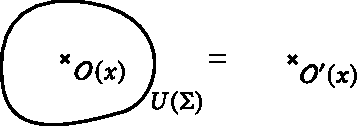
\includegraphics{EgWTid.pdf}
\end{align}
というようなものがあります。これは$x$は時空の点で$\Ocal(x),\Ocal'(x)$は局所演算子、$\Sigma$は余次元1の面で$U(\Sigma)$は$\Sigma$に局在した演算子(欠陥)です。この「式」の意味は
\begin{align}
  \expval{U(\Sigma)\Ocal(x)\cdots}=\expval{\Ocal'(x)\cdots},\qquad&(\text{$\cdots$は両辺で共通の任意の演算子の挿入。 }\notag \\
  &\text{ただし、$\cdots$は$\Sigma$の内側には挿入されていない。})
\end{align}
という意味です。

\end{document}